\section{Experiments and results}
\label{section-experiments}

\subsection{Tool descriptions}

\noindent\textbf{\GROOVE.}
Rensink \cite{rensink2009:isomorphism,rensink2007:isomorphism} uses an
isomorphism invariant hash code combined with one-to-one isomorphism checking
for symmetry reduction in model checking. For state graphs an invariant hash
code is computed. This hash code is used as key for the graph in the state
store, which is implemented as a hash map. In order to check if a state has been
visited before, the hash value is computed and only the graphs at the associated
position in the hash map are compared to the newly encountered state. This
reduces the number of graphs that have to be compared (by a factor that depends
on the quality of the hash function). The hash code is based on a partition
refinement algorithm where similar nodes are in the same cell. Each cell is
distinguished by the number of incoming and outgoing edges and associated labels
of nodes and those of the neighbouring nodes.

\medskip\noindent\textbf{\NAUTY and \BLISS.}
The canonical form of a graph is computed by \NAUTY and \BLISS by generating for
each graph a set of discrete partitions that can be used as a permutation of the
nodes of the graph. Given some ordering of the graphs, we can choose the minimum
or maximum of the set as the canonical form if the same set of permuted graphs
is generated for isomorphic graphs. \NAUTY and \BLISS use efficient algorithms
that avoid generating all possible node permutations, but still result in an
equal set of permuted graphs for isomorphic graphs. The algorithms mainly
consist of the following two ingredients:
\begin{inparaenum}
\item a partition refinement algorithm that computes the unique coarsest stable
partition for a given graph and initial partition of nodes;
\item an algorithm that generates a search tree of stable partitions with
discrete partitions as leaf nodes, of which one is chosen as the relabelling
partition permutation leading to the canonical form.
\end{inparaenum}

The search tree is generated by first computing a stable partition (which is the
root node of the tree) and then splitting one of the cells. For each of the
members of the cell a subtree is added, where that member is put in a separate
cell. Then each of the resulting partitions is stabilised again. This continues
until all branches end in discrete partitions (the leaf nodes). Because every
intermediate partition is stabilised before it is split again, the number of
nodes in the tree is reduced. The properties that are used in the partition
refinement are isomorphism invariant, so the resulting set of permuted graphs
stays equal for isomorphic graphs.

\subsection{Experiment setup}

\subsubsection{Combinations of tools and conversions.}
The combinations of isomorphism checking tools and conversion methods included
in the experiments are:
\begin{description}\itemsep0pt
\item[\GROOVE] The algorithm that is already implemented in \GROOVE, which
checks if two edge-labelled graphs are isomorphic;
\item[Layered-\BLISS] Conversion function $\tau_1$ combined with the tool
\BLISS.
\item[Layered-\NAUTY] Conversion function $\tau_1$ combined with the tool
\NAUTY.
\item[Edgenode-\BLISS] Conversion function $\tau_2$ combined with the tool
\BLISS.
\item[Edgenode-\NAUTY] Conversion function $\tau_2$ combined with the tool
\NAUTY.
\end{description}

\subsubsection{Graphs.}
We chose a set of 10 graphs of various sizes that are used as state graphs
in model checking. For each of these graphs, we have an isomorphic variant and
a non-isomorphic but otherwise similar one.
\begin{description}
\item[no-hops-*] States in the model of an ad-hoc network connectivity protocol
that is described and used in \cite{rensink2009:isomorphism}. The graphs used
here have four or seven nodes in the network and a designated scheduler node.
The graphs are quite symmetric.
\item[circ-buffer-3] State in a model of a circular buffer with three cells.
\item[din-phil-*] States in a model of the philosophers problem with three
philosophers.
\item[checkers-s*] States of the checkers boardgame. The graphs are not very
symmetric, because several different labels are used to distinguish places on
the board.
\item[seq3-flow2] A large and mildly dense graph modelling a sequence of
actions in a program. The graph is not very symmetric.
\end{description}

\subsubsection{Experiment environment.}
The experiments were performed on a system with two Quad Core Xeon 1.86GHz
CPU's and 8GB of memory running openSUSE 10.2 with Linux kernel 2.6.27 (64 bit).
\GROOVE version 3.3.1 was used with a Java 1.6.0 VM with a maximum of 3640 MB of
memory. \NAUTY version 2.4b7 \cite{mckay2008:nauty24} and \BLISS version 0.50
\cite{junttila2008:bliss} were employed.

The experiments involved pair-wise comparison of the edge-labelled graphs
given above for isomorphism. When using a graph conversion, the edge-labelled
graphs are first converted to a node-coloured graph and their canonical forms
are computed, then these canonical forms are checked for equality. \GROOVE
checks for isomorphism of two edge-labelled graphs directly. Each experiment was
performed 10 times and we give the average execution time. Since most tools
finish within seconds and we are interested in algorithms that are fast,
experiments lasting longer than 5 minutes were aborted.

\subsection{Results}

Table~\ref{table:conversion} present information about the size of the graphs
used. Lines marked with $|V|$ and $|E|$ indicate the number of nodes and edges
of a graph, respectively. For each conversion method we give the conversion
time in {\it ms}. From the table we see that the layered conversion yields
smaller graphs only when the original graph is very small ($< 10$ nodes). On the
other cases the edge node conversion is clearly better.

\begin{table}[!tbp]
\caption{Results for the conversion methods. Time is in {\it ms}.}
\centering
\begin{tabular}{l@{\enspace} c @{\enspace} | @{\enspace}r @{\enspace}r
@{\enspace}r @{\enspace}r @{\enspace}r @{\enspace}r @{\enspace}r @{\enspace}r
@{\enspace}r @{\enspace}r}
& & \rotatebox{90}{no-hops-4} & \rotatebox{90}{no-hops-7} &
\rotatebox{90}{circ-buf-3} & \rotatebox{90}{din-phil-0} &
\rotatebox{90}{din-phil-1} & \rotatebox{90}{checkers-s144} &
\rotatebox{90}{checkers-s5} & \rotatebox{90}{checkers-s62} &
\rotatebox{90}{checkers-s1} & \rotatebox{90}{seq3-flow2} \\
\hline
Original & $|V|$ & 5 & 8 & 4 & 6 & 6 & 70 & 69 & 70 & 117 & 75 \\
graph & $|E|$ & 15 & 45 & 9 & 12 & 13 & 294 & 309 & 303 & 357 & 549 \\
\hline
Layered & $|V|$ & 5 & 8 & 12 & 12 & 18 & 630 & 621 & 630 & 1,053 & 1,725 \\
conversion & $|E|$ & 8 & 35 & 13 & 12 & 19 & 782 & 791 & 792 & 1,175 & 1,858 \\
$\tau_1$ & time & 0.5 & 0.8 & 0.4 & 0.4 & 0.5 & 3.6 & 2.7 & 2.0 & 3.1 & 6.4 \\
\hline
Edge node & $|V|$ & 13 & 43 & 9 & 12 & 13 & 292 & 308 & 302 & 356 & 283 \\
conversion & $|E|$ & 16 & 70 & 10 & 12 & 14 & 444 & 478 & 464 & 478 & 416 \\
$\tau_2$ & time & 0.6 & 1.0 & 0.3 & 0.3 & 0.3 & 2.3 & 1.3 & 1.0 & 1.4 & 1.2\\
\hline
\end{tabular}
\label{table:conversion}
\end{table}

\begin{table}[!tbp]
\caption{Results for the experiments performed. Time is in {\it ms}.}
\centering
\begin{tabular}{l@{\enspace} r@{\enspace} | @{\enspace}r @{\enspace}r
@{\enspace}r @{\enspace}r @{\enspace}r @{\enspace}r @{\enspace}r @{\enspace}r
@{\enspace}r @{\enspace}r}
& & \rotatebox{90}{no-hops-4} & \rotatebox{90}{no-hops-7} &
\rotatebox{90}{circ-buf-3} & \rotatebox{90}{din-phil-0} &
\rotatebox{90}{din-phil-1} & \rotatebox{90}{checkers-s144} &
\rotatebox{90}{checkers-s5} & \rotatebox{90}{checkers-s62} &
\rotatebox{90}{checkers-s1} & \rotatebox{90}{seq3-flow2} \\
\hline
\multirow{5}{*}{\rotatebox{90}{Iso}}
& \GROOVE & 5.3 & 9.7 & 2.4 & 3.3 & 2.2 & 9.9 & 5.0 & 6.4 & 14.7 & 6.9 \\
& Layered-\BLISS & 6.5 & 8.3 & 5.4 & 9.5 & 6.0 & 27.4 & 22.2 & 22.1 & 30.5 &
53.1 \\
& Layered-\NAUTY & 5.7 & 9.0 & 5.7 & 4.9 & 8.3 & 9,303.9 & -- & -- & -- & -- \\
& Edgenode-\BLISS & 10.5 & 13.8 & 4.1 & 4.5 & 4.6 & 17.7 & 13.0 & 12.2 & 13.2 &
12.1 \\
& Edgenode-\NAUTY & 7.9 & -- & 6.9 & 6.7 & 5.2 & -- & -- & -- & -- & -- \\
\hline
\multirow{5}{*}{\rotatebox{90}{Non-iso}}
& \GROOVE & 4.1 & 7.5 & 2.0 & 3.4 & 2.3 & 8.7 & 5.6 & 5.3 & 12.0 & 4.7 \\
& Layered-\BLISS & 7.3 & 10.3 & 5.3 & 5.5 & 6.2 & 29.0 & 21.1 & 20.8 & 31.9 &
51.9 \\
& Layered-\NAUTY & 6.4 & 6.5 & 6.3 & 4.7 & 5.1 & -- & -- & -- & -- & -- \\
& Edgenode-\BLISS & 10.2 & 16.5 & 4.2 & 4.5 & 7.0 & 17.2 & 13.0 & 11.6 & 13.2 &
12.0 \\
& Edgenode-\NAUTY & 10.4 & -- & 6.9 & 6.0 & 4.7 & -- & -- & -- & -- \\
\hline
\end{tabular}
\label{table:results}
\end{table}

The running times for the tools are in Table~\ref{table:results}. We see that
there is not much difference in execution time between isomorphic and
non-isomorphic pairs of graphs. From the results we see that \NAUTY does well
for some small graphs, but is unable to give an answer within 5 minutes for the
larger graphs. \BLISS with the label-node conversion ($\tau_2$) is the
conversion method that perform closest to \GROOVE but still is usually two times
slower, except for the largest graph (checkers-s1). Performance is clearly
related to the size of the graph after conversion. For the isomorphic graphs,
Fig.~\ref{fig:plot} gives plots of the values in Table~\ref{table:results}.

\begin{figure}[!tbp]
\begin{center}
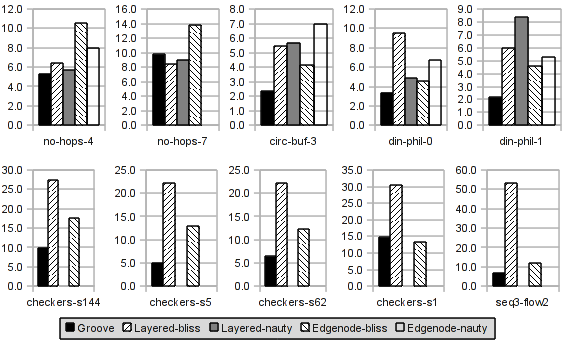
\includegraphics[scale=0.6]{images/plot.png}
\caption{Plots for the execution time of isomorphic pairs of graphs.}
\label{fig:plot}
\end{center}
\end{figure}
